\documentclass[9pt,twocolumn,twoside]{pnas-new}
% Use the lineno option to display guide line numbers if required.
% Note that the use of elements such as single-column equations
% may affect the guide line number alignment. 

\templatetype{pnasresearcharticle} % Choose template 
% {pnasresearcharticle} = Template for a two-column research article
% {pnasmathematics} = Template for a one-column mathematics article
% {pnasinvited} = Template for a PNAS invited submission

\usepackage{amsmath}
\usepackage{subcaption}
\usepackage{gensymb}

\setboolean{displaywatermark}{false}

\title{Perturbing the catalase active site electric field via genetic code expansion}

% Use letters for affiliations, numbers to show equal authorship (if applicable) and to indicate the corresponding author
\author[a,1,2]{Elliott Capek}
\author[a]{Laikana Ly}
\author[a]{Hassan Alnatah}
\author[a]{Joey Orton}
\author[a]{Aiden Estelle}

\affil[a]{Oregon State University Department of Biohchemistry and Biophysics}

% Please give the surname of the lead author for the running footer
\leadauthor{Capek}

% Please include corresponding author, author contribution and author declaration information
\equalauthors{\textsuperscript{1} Author wrote the manuscript.}
\correspondingauthor{\textsuperscript{2}To whom correspondence should be addressed. E-mail: capeke\@ oregonstate.edu}

% Keywords are not mandatory, but authors are strongly encouraged to provide them. If provided, please include two to five keywords, separated by the pipe symbol, e.g:
\keywords{Noncanonical amino acid $|$ catalase $|$ electric field $|$ active site} 

\begin{abstract}
  Catalase is a ubiquitous enzyme which breaks down hydrogen peroxide into oxygen gas and water. Numerous theories exist about how catalase achieves its high catalytic efficiency. One theory is that an electric field within catalase's active site orients the dipole moments of substrate optimally to react with heme. Here we demonstrate how genetic code expansion can be used to purturb the electric field within catalase. We do so by replacing Phe 206 with 3-nitrotyrosine (3NY). We find that this mutation doubles Michaelis constant $K_M$ to $571$ mmol, compared to wildtype $245$ mmol. Mutant Michaelis constant $kcat$ goes down by a factor of 100 to $300 s^{-1}$, compared to wildtype $36,100 s^{-1}$. By switching 3NY's protonation state by conducting kinetic assays at high and low pH, we find charge on 3NY significantly effects enzyme velocity. At high pH the initial velocity is roughly half the low-pH velocity.
\end{abstract}

%% \dates{This manuscript was compiled on \today}
\doi{\url{www.pnas.org/cgi/doi/10.1073/pnas.XXXXXXXXXX}}

\begin{document}

% Optional adjustment to line up main text (after abstract) of first page with line numbers, when using both lineno and twocolumn options.
% You should only change this length when you've finalised the article contents.
\verticaladjustment{-2pt}

\maketitle
\thispagestyle{firststyle}
\ifthenelse{\boolean{shortarticle}}{\ifthenelse{\boolean{singlecolumn}}{\abscontentformatted}{\abscontent}}{}

% If your first paragraph (i.e. with the \dropcap) contains a list environment (quote, quotation, theorem, definition, enumerate, itemize...), the line after the list may have some extra indentation. If this is the case, add \parshape=0 to the end of the list environment.
\dropcap{C}atalase is an enzyme which catalyzes the breakdown of hydrogen peroxide into water and oxygen gas. This is an important detoxification reaction, since hydrogen peroxide is a reactive toxin generated by several biological processes. Catalase is a tetrameric protein which uses a heme group in its active site to facilitate the breakdown of hydrogen peroxide. The molecular mechaninism of catalase proceeds in two steps. First, the heme reduces a hydrogen peroxide, producing water and the so-called Cpd I. Then Cpd I oxidizes a second hydrogen peroxide, producing water and oxygen gas. This second step is mediated by a histidine near the active site \cite{alfonso-prieto}.\\

One remaining question about catalase is how it achieves its remarkable speed given its buried active site. The enzyme is nearly diffusion-limited\cite{kcatkm, difflimit}, indicating it turns substrate to product at close to the optimal rate. However, in order to reach the active site, hydrogen peroxide must diffuse through a 30 $\AA$ tunnel\cite{substrateflow}. Thus, substrate must be transported very efficiently through the protein. Understanding how this transport process works could provide lots of insight into how enzymes traffic substrate into buried active sites. Catalase is one of the most studied proteins in existence, and so represents a good model protein for understanding substrate trafficking.\\

Previous work on substrate trafficking has illuminated various stages in the process. The enzyme has a number of high-H2O2-residency surface residues, which are believed to concentrate the substrate near the entrance to the active channel \cite{concentrateh2o2}. The active channel itself seems optimized to maximize substrate flow, to the point that mutagenesis to open the channel decreases enzyme activity \cite{substrateflow}. The channel seems to be capable of selecting the molecules which enter it using a patch of hydrophobic residues which are situated to preferentially pass the bulkier H2O2 \cite{molecularruler}. Even the directionality of substrate within the channel seems to be controlled: one channel is used for substrate entrance, and the other for product exit \cite{lateralchannel}. However, how substrate is traficked once in the active site antechamber is still an open question.\\

One tool proteins are known to use to speed up active site kinetics is the use of electric fields. Superoxide dismutase is known to have a strong E-field in its active site to stabilize dipolar intermediates \cite{conserved-as-efield-sod, concentrated-as-efield-sod}. Several other proteins are known to use a similar effect \cite{efield-review} (be more precise here). It has been suggested that catalase uses an electric field in its active site to orient and traffick hydrogen peroxide to its active heme \cite{electricpotential}. This model, proposed by Chelikani \textit{et. al}, theorizes that a strong electric field from the negative asparigine 181 at the top of the active site antechamber extends to the strongly positive heme iron, as shown in Figure \ref{fig:hypothesis}.d. This electric field would orient incoming hydrogen peroxides in the optimal rotation for reaction with heme.\\

An issue with mutagenesis studies like Chelikani \textit{et. al.} is that catalase's active site is very sensitive to changes. Replacing residues in the active site can dramatically impact enzyme efficiency \cite{substrateflow}. A better technique would purturb the electric field without full amino acid mutagenesis. Here we propose a new method for studying the catalase active site: genetic code expansion. We demonstrate how noncanonical amino acids can be incorporated into the catalase active site, as described in \textit{Hamill et. al.}, and how these modifications allow a less drastic change in active site environment. We use genetic code expansion \cite{hammill} to incorporate two functional groups onto F206 in the catalase active site, turning it into 3-nitrotyrosine (Figure \ref{fig:hypothesis}.e). This change is important because it a.) is tiny, adding only 30 $\AA^3$ of steric bulk \cite{3ntsize}, and b.) incorporates a hydroxy group of pKa 7.0 into the catalase active site \cite{3ntsize}. Catalase activity is pH-invariant in the range of 5 to 9 \cite{phdependence,kcatkm}; thus, by incorporating a group which gains charge at pH 7, we can precisely study the effect of charge in the catalase active site on enzyme kinetics without worrying about the undesired effects of mutagenesis.\\

\begin{figure*}
  \includegraphics[width=0.24\linewidth]{figures/cartoon-visualization.png}
  \includegraphics[width=0.24\linewidth]{figures/channel-visualization.png}
  \includegraphics[width=0.24\linewidth]{figures/efield-wt.pdf}
  \includegraphics[width=0.24\linewidth]{figures/efield-3ny.pdf}%
  \caption{Depiction of catalase active pocket. \textbf{Left:} wildtype pocket with proposed ligand-orienting E-field \cite{electricpotential}. The field should orient H2O2 for optimal reaction with the heme. \textbf{Right:} modified HPII-3NY with a deprotonated 3-nitrotyrosine residue at site 206, with hypothetical augmented E-field. The disrupted E-field should result in un- or mis-aligned substrate.}
  \label{fig:hypothesis}
\end{figure*}

\begin{figure}
  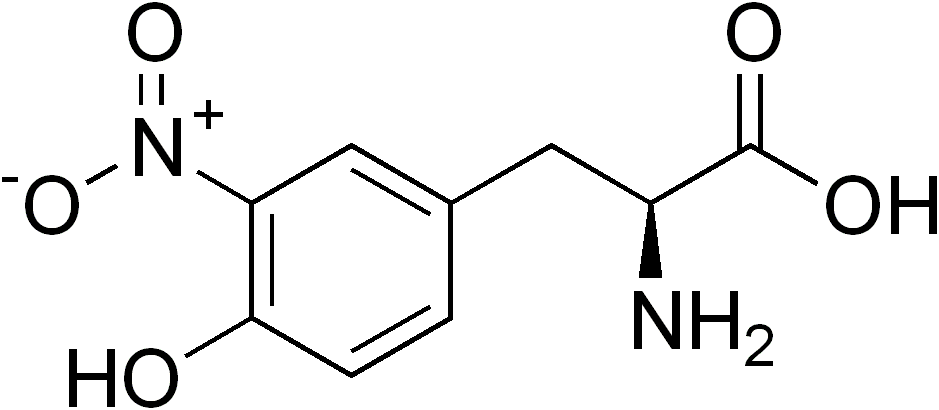
\includegraphics[width=0.4\linewidth]{figures/3ny.png}
  \hspace{0.1\linewidth}
  
\includegraphics[width=0.5\linewidth]{figures/pazf.png}
  \caption{\textbf{Structures of two noncanonical amino acids used in study.} \textit{Left:} 3-nitrotyrosine, \textit{Right:} para-azidophenylalanine.}
\end{figure}

\section{Results}
%% to add: Chemical nature and location of your ncAAs in the structure. (This might fit best in results).
Noncanonical amino acids (ncAAs) were incorporated into protein constructs by mutating the desired codon to TAG, then adding TAG-recognizing ncAA-tRNA synthetases and compatible tRNAs to cells. His-tagged protein constructs were grown in DH10 \textit{E. coli} and purified using TALON metal affinity resin. An SDS-PAGE gel of purified protein is shown in Figure \ref{fig:pure-gel}. HPII is expected to be in its 84-kD monomeric state in the denaturing and reducing conditions of SDS-PAGE; an 80kD band is seen for all three purified HPII constructs. This verifies that HPII-ncAA cells properly produce noncanonical aminoacyl-tRNA, which is the only tRNA which recognizes the TAG codon and allows for full-length protein translation. Contaminant bands in the gel are faint but visible, suggesting protein of $\approx$ 90\% purity. ncAA-incorporated proteins were grown with and without ncAA to verify proper incorporation. Without ncAA, cells should lack any aminoacyl-tRNA for the TAG codon, and thus HPII-ncAA peptides should stall on the ribosome, resulting in truncated peptides of approximately 22kD. This is seen in Figure \ref{fig:pure-gel}, where HPII-ncAA lanes lacking ncAA lack a 80kD band but do have bands of approximately 25kD.\\

\begin{figure}
  \centering
  \includegraphics[width=\linewidth]{figures/gene-diagram}
  \includegraphics[width=\linewidth]{figures/plasmid-diagram}
  \caption{\textbf{Design of protein constructs and expression plasmids} \textit{top:} genes of three constructs used in study. \textit{bottom:} pBad and pDule plasmids.}
  \label{fig:design}
\end{figure}

\begin{figure}
  \centering
  \includegraphics[width=\linewidth]{figures/pure-gel}
  \caption{\textbf{Electrophoresis gel of crude lysate and purified protein expression.} \textbf{a.} Gene constructs used. \textbf{b.} Plasmid schematics for relevant plasmids. Amp$^R$ and Tet$^R$ are antibiotic resistance genes, Nitro-Y-RS and pCNF-RS are tRNA synthases compatible with 3-nitrotyrosine and p-azido-l-phenylalanine, and tRNA$_{CUA}$ is a tRNA compatible with the respective synthase. \textbf{c.}Major band in purification lanes correspond to protein of approximately 80kD, as expected for a catalase single subunit. Crude negative control lanes lack 80kD band, consistent with noncanonical amino acid being necessary for noncanonical protein expression. Crude negative control lanes have smaller protein bands, consistent with truncated protein formation.}
  \label{fig:pure-gel}
\end{figure}

\begin{figure}
  \centering
  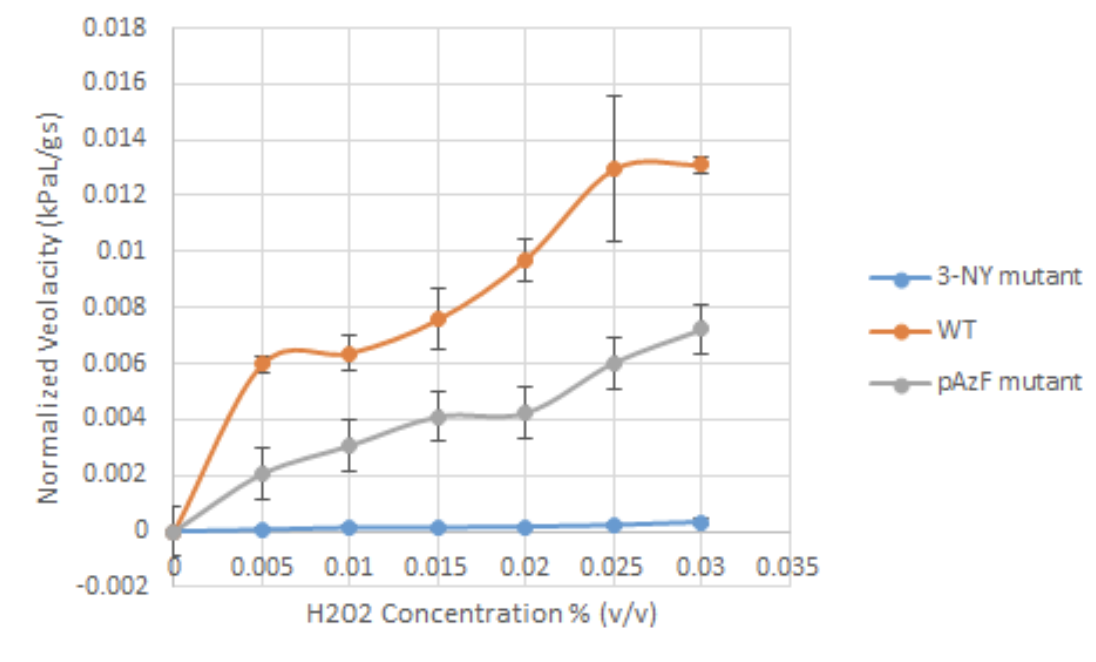
\includegraphics[width=0.9\linewidth]{figures/kinetics.png}
  \begin{tabular}{lll}
      \hline
      Sample  & $K_M$ (M) & kcat ($s^{-1}$) \\
      \hline
      HPII        & $1.3$ & $2.3x10^6$\\
      HPII-3NY    & $1.4$ & $6.9x10^6$\\
      HPII-pAzF   & $1.7$ & $2.2x10^5$\\
      \hline
  \end{tabular}
  \caption{\textbf{Michaelis-Menten plot of kinetic efficiencies of HPII variants.} Kinetic measurements conducted at 25\degree C using the pressure-based assay defined above.}
  \label{fig:kinetics}
\end{figure}

\begin{figure}
  \centering
  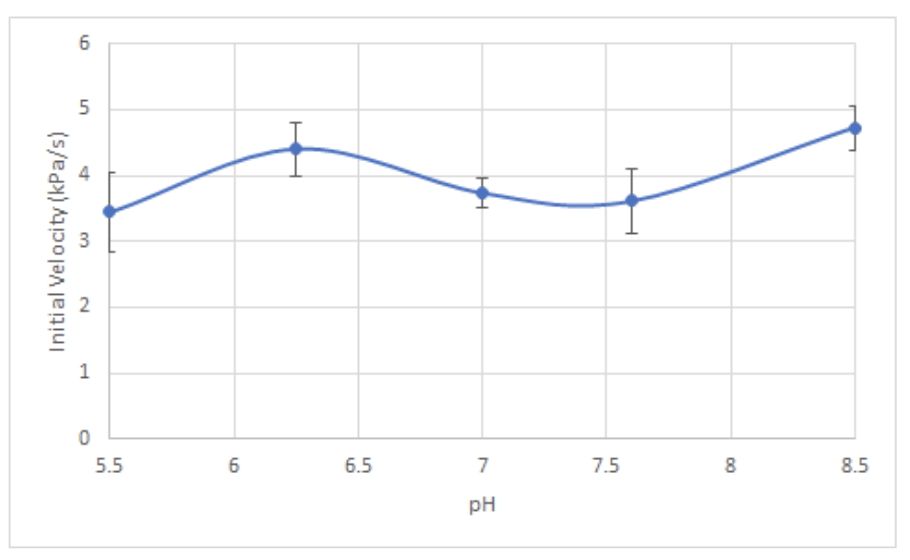
\includegraphics[width=0.9\linewidth]{figures/wildtype-velocity.png}
  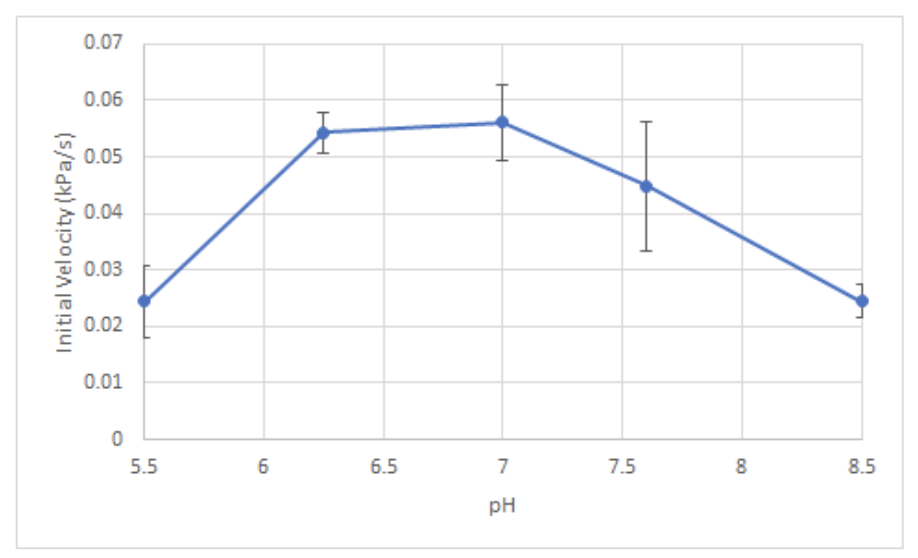
\includegraphics[width=0.9\linewidth]{figures/3ny-velocity.png}
  \caption{\textbf{pH dependent initial velocities of HPII variants.} Left: HPII catalase Right: HPII-3NY.}
  \label{fig:ph-dependent-velocities}
\end{figure}

\subsection*{Discussion}

\subsection*{Conclusion}

ncAA substitution is a powerful technique which allows easy testing of hypotheses in regions which are very sensitive to structural change. This technique could be used to test -other-catalase-hypotheses-.\\

Perhaps this technique could be used to study e-fields generally.\\

We propose that the following residues be incorporated into the channel at sites - - -. Coupled with APBS simulations, these results could be a powerful test of the effects of catalase e-field.\\

\matmethods{

\subsection*{Protein production}
Wildtype protein was expressed by transforming the plasmid pBad-HPII (Fig \ref{fig:protein-design}.b, modified from Addgene ID 105839), containing WT HPII gene, into competent \textit{E. coli} DH10B cells via heat-shock. pBad-HPII plasmid includes ampicillin resistance, an arabinose-induced promoter, and a 6xHis codon sequence on the N-term of the HPII gene. Cells were then grown in autoinduction media with an arabinose inducer (0.1\% aspartate, 0.2\% glycerol, 100$\mu g / mL$ ampicillin, mineral salts, 0.05\% glucose, 20mM MgSO4, 0.05\% arabinose, trace metals and amino acid mix, pH 7.5) for 48 hours, shaking, at 37\degree C. Cells were then pelletized and stored at -80\degree C.\\

The same protocol was followed for the ncAA mutant catalases HPII-3NY and HPII-pAzF, except using protein plasmids pBad-HPII-3NY and pBad-HPII-pAzF (Addgene ID 105846) instead. ncAA tRNA synthase plasmids pDule-Nitro-RS and pDule-pCNF-RS (Fig \ref{fig:protein-design}.b, modified from Addgene ID 85498), which contain a tetracycline resistance gene, a TAG tRNA, and a compatible tRNA synthase, were also transformed into DH10B. ncAA autoinduction media was supplemented with $25\mu g / mL$ tetracycline to select for both plasmids.\\

$OD_{600}$ measurements of cultures at 48 hours growth time were 0.65, 0.58 and 0.45 optical density for HPII, HPII-3NY and HPII-pAzF expressions.\\

\subsection*{Protein purification}
Pelletized cells were reconstituted in TALON equilibration buffer (50mM sodium phosphate, 300mM NaCl, pH 7.0) and microfluidized, also in equilibration buffer. Lysed cells were spun down at 15K RPM for 20 minutes at 4\degree C. Supernatant was collected and combined with 300$\mu L$ bed volume TALON beads per 100mL cultured cells. TALON-supernatant mix was nutated for 30 minutes at 4\degree C. Bound beads were then spun down at 500g for 5 minutes and the supernatant discarded. The beads were applied to a pre-washed gravity-flow column at room temperature and washed twice with 10mL equilibration buffer. Elution was done using 2mL elution buffer (50mM sodium phosphate, 300mM NaCl, 250mM imidazole, pH 7.0) into four 500$\mu L$ aliquots. Protein was not desalted. Protein was then stored at 4\degree C.\\

\subsection*{Concentration determination}
A Bio-Rad Bradford assay kit was employed using the standard protocol. Bovine serum albumin was used as the reference protein to construct the standard curve. Concentrations from 125 $\mu g / mL$ to 2 mg/mL were explored. Samples were incubated with dye in cuvettes for 5 minutes at room temperature. Samples were then analyzed via spectrophotometer at 595 \textit{nm} and used to create the standard curve. HPII protein samples were then compared to this standard curve to estimate their concentration.\\

\subsection*{Activity assessment}
Enzyme velocity was measured using a Vernier Gas Pressure Sensor. Reaction buffer (50mM sodium phosphate, 300mM NaCl, 5\% $H_2O_2$ pH modulated to 5.5, 6.25, 7.0, 7.75, 8.5 via addition of HCL or NaOH) was combined with enzyme (25 $\mu g/mL$, 50 $\mu g/mL$, 50$\mu g/mL$ for HPII, HPII-3NY, HPII-pAzF) to a total volume of $3mL$ in pressure sensor tube. Tubes were sealed and pressure was monitored at 1s intervals for 120 seconds. Data was collected using Vernier LoggerPro.\\

\subsection*{pH dependent assay}
pH assays were conducted using the same kinetic method described above. Reactions occured in 3mL equilibration buffer (50mM sodium phosphate, 300mM NaCl, 5\% $H_2O_2$ pH modulated to values from 5 to 10 via addition of HCL or NaOH). On addition of 43$\mu g$ protein, the tubes were mixed and incubated at RT for five minutes, then brought to 5\% $H_2O_2$ and added to pressure assay mechanism. Trials were conducted in triplicate.\\
}

\showmatmethods % Display the Materials and Methods section

% \pnasbreak splits and balances the columns before the references.
% If you see unexpected formatting errors, try commenting out this line
% as it can run into problems with floats and footnotes on the final page.
\pnasbreak

% Bibliography
\bibliography{references}

\end{document}
